\documentclass[]{beamer}
% Class options include: notes, notesonly, handout, trans,
%                        hidesubsections, shadesubsections,
%                        inrow, blue, red, grey, brown

\usepackage{graphicx}
\usepackage{booktabs}
\usepackage{tikz}

\usetheme{Madrid}
\usecolortheme{dolphin}
%\usecolortheme{seagull}
%\usecolortheme{seahorse}
\useoutertheme{infolines}
\useinnertheme{rectangles}
%\useoutertheme[footline=authortitle]{miniframes}

\setbeamercolor{block title}{bg=blue}
%\setbeamerfont*{title}{size=\huge}

% Theme for beamer presentation.
%\usepackage{beamerthemesplit} 
%\usepackage{beamerthemelined} 
% Other themes include: beamerthemebars, beamerthemelined, 
%                       beamerthemetree, beamerthemetreebars  

\beamertemplatenavigationsymbolsempty

\makeatletter
\setbeamertemplate{footline}
{
  \leavevmode%
  \hbox{%
  \begin{beamercolorbox}[wd=\paperwidth,ht=2.25ex,dp=1ex,right]{date in head/foot}%
    \usebeamerfont{date in head/foot}\insertshortdate{}\hspace*{2em}
    \insertframenumber{} / \inserttotalframenumber\hspace*{2ex} 
  \end{beamercolorbox}}%
  \vskip0pt%
}
\makeatother

%\setbeamercolor*{title}{bg=gray,fg=blue}
\title{Managing Relationships\\between Code and Documentation}    % Enter your title between curly braces
\author{Dejun Qian}                 % Enter your name between curly braces
\institute{Portland State University}      % Enter your institute name between curly braces
%\date{\today}                    % Enter the date or \today between curly braces
\date{}                    % Enter the date or \today between curly braces

\begin{document}

% Creates title page of slide show using above information
\begin{frame}
  \titlepage
\end{frame}
\note{Good afternoon, everyone. My name is Dejun Qian. Today I will talk about how to manage relationships between code and documentation.}

%\section[Outline]{}

% Creates table of contents slide incorporating
% all \section and \subsection commands
%\begin{frame}
%  \frametitle{Agenda}
%  \tableofcontents
%\end{frame}


\section{Background}
\subsection{Code vs Documentation}
\begin{frame}{\centerline{Background}}
  \includegraphics[width=\textwidth]{problem1}
\end{frame}
\note{To write and maintain code efficiently, we need documentation. Usually, code is composed of several code files, and each code file contains a string of ASCII charactors. Basically the string conforms to the syntax of certain languages like C, Java, and etc.. Compared to code, documentation is much more complicated. It may be in different file formats, like pdf, html, MS word, and etc.. Instead of raw ASCII string, the content in documentation could be text, table, picture, and etc..}

\subsection{Relationships}
\begin{frame}{\centerline{Background}}
  \includegraphics[width=\textwidth]{problem2}
\end{frame}
\note{Usually, just knowing which documentation file is needed for which code file does not help too much. We need more detailed information. As we read code word by word, and line by line, we need to know which code segment is related to which document segment.}

\section{Problem Statement}
\subsection{Problems}
\begin{frame}[b]{\centerline{Problem}}
  \ \\
  \fontsize{13.5}{11}\selectfont How to represent the code segments with
  \begin{itemize}
  \item code-evolving invariance,
  \item flexible granularity,
  \item and non-ambiguity? %\normalsize
  \end{itemize}
  \begin{center}
  \includegraphics[width=.9\textwidth]{problem3}
  \end{center}
\end{frame}
%\note[enumerate]       % Add notes to yourself that will be displayed when
%{                      % typeset with the notes or notesonly class options
%\item Note for Point 1   
%\item Note for Point 2   
%}


\section{Previous Solution}
\subsection{Previous Solutions}
\begin{frame}{\centerline{Previous Work}}
  \ \\
  \fontsize{13.5}{11}\selectfont
  \begin{itemize}
  \item Comment-based representation
    \begin{itemize}
      \item Javadoc uses this to write documentation for code segments.
    \end{itemize}
  \ \\
  \ \\
  \item Offset-based representation
    \begin{itemize}
      \item Compiler uses this method to highlight error code.
    \end{itemize}
  \end{itemize}
\end{frame}

\subsection{Comment-Representation}
\begin{frame}
  \frametitle{\centerline{Comment-Based Representation}}
  \fontsize{13.5}{11}\selectfont
  \begin{columns}[c]
  \column{2.5in}  % slides are 3in high by 5in wide
  Advantage
  \begin{itemize}
  \item Code-evolving invariance
  \end{itemize}
  \vspace{2em}
  Disadvantage
  \begin{itemize}
  \item Coarse granularity
  \item Ambiguity
  \end{itemize}
  \column{1.5in}
  \includegraphics[height=.9\textheight]{comment}
  \end{columns}
\end{frame}

\subsection{Offset-Representation}
\begin{frame}
  \frametitle{\centerline{Offset-Based Representation}}
  \fontsize{13.5}{11}\selectfont
  \begin{columns}[c]
  \column{2in}  % slides are 3in high by 5in wide
  Advantage
  \begin{itemize}
  \item Flexible granularity
  \item No ambiguity
  \end{itemize}
  \vspace{2em}
  Disadvantage
  \begin{itemize}
  \item No code-evolving invariance
  \end{itemize}
  \column{2in}
  \includegraphics[height=.9\textheight]{offset}
  \end{columns}
\end{frame}


\section{Solution}
\subsection{Abstract Syntax Tree}
\begin{frame}
  \frametitle{\centerline{Abstract Syntax Tree}}
  \begin{columns}[c]
  \column{1.8in}  % slides are 3in high by 5in wide
  \includegraphics[width=.9\textwidth]{code1}
  \column{2.5in}
  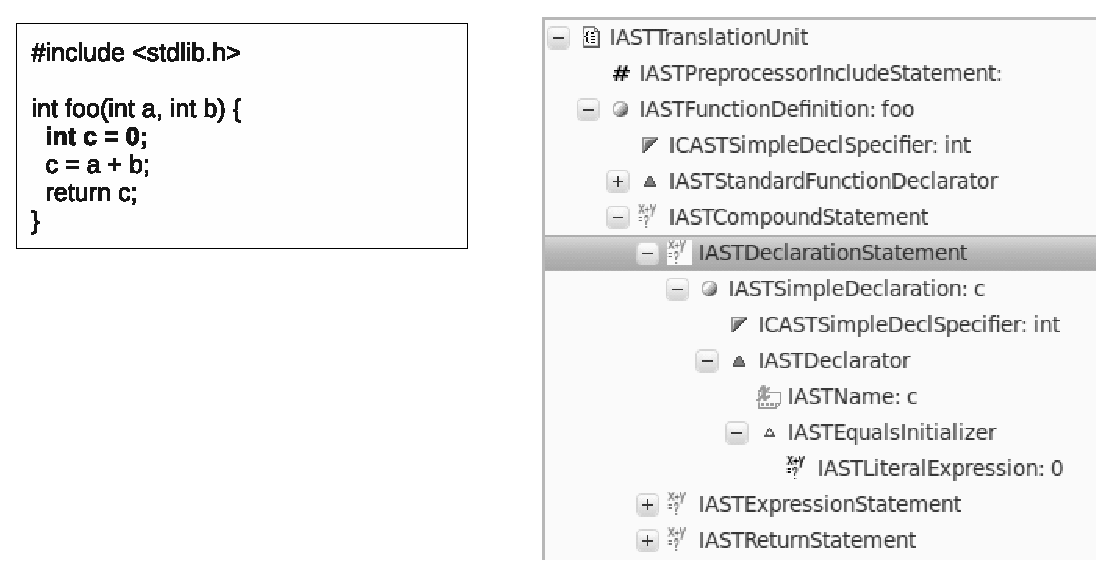
\includegraphics[height=.75\textheight]{ast1}
  \end{columns}
\end{frame}
\note{The end}

\subsection{Code-evolving Invariance}
\begin{frame}
  \frametitle{\centerline{AST-Based Representation}}
  \begin{columns}[c]
  \column{1.8in}  % slides are 3in high by 5in wide
  \includegraphics[width=.9\textwidth]{code11}
  \column{2.5in}
  \includegraphics[height=.75\textheight]{ast11}
  \end{columns}
\end{frame}


%\subsection{Code-evolving Invariance}
%\begin{frame}[b]
%  \frametitle{\centerline{Code-evolving Invariance}}
  %\begin{center}
%  \begin{tikzpicture}
%    \node (img1) {\includegraphics[height=.75\textheight]{code21}};
    %\pause
%    \node (img2) at (img1.east)[xshift=.1\textheight] {\includegraphics[width=.95\textwidth]{ast21}};
%  \end{tikzpicture}
  %\end{center}
  %\includegraphics[width=.9\textwidth]{code21}
  %\includegraphics[height=.75\textheight]{ast21}
%\end{frame}

\subsection{Code-evolving Invariance}
\begin{frame}
  \frametitle{\centerline{Code-evolving Invariance}}
  \begin{columns}[c]
  \column{1.8in}  % slides are 3in high by 5in wide
  \includegraphics[width=.9\textwidth]{code21}
  \column{2.5in}
  \includegraphics[height=.75\textheight]{ast22}
  \end{columns}
\end{frame}

\subsection{Granularity}
\begin{frame}
  \frametitle{\centerline{Granularity and Non-ambiguity}}
  \begin{columns}[c]
  \column{1.8in}  % slides are 3in high by 5in wide
  \includegraphics[width=.9\textwidth]{code23}
  \column{2.5in}
  \includegraphics[height=.75\textheight]{ast23}
  \end{columns}
\end{frame}
\note{The end}

\section{Preliminary Result}
\subsection{Preliminary Result}
\begin{frame}{\centerline{Preliminary Result}}
  \begin{center}
  \includegraphics[width=.9\textwidth]{platformview}
  \end{center}
\end{frame}

\subsection{Preliminary Result}
\begin{frame}[b]{\centerline{Preliminary Result}}
  \fontsize{13.5}{11}\selectfont
  \begin{itemize}
  \item Preserve all the relationships after code evolves.
  \item Provide flexible granularity and non-ambiguity.
  \end{itemize}
  \centerline{\includegraphics[width=.7\textwidth]{platformview}}
\end{frame}

\section{Conclusion}
\begin{frame}[t]{\centerline{Conclusion}}
  \ \\
  \fontsize{10}{11}\selectfont
  \centerline{
  \begin{tabular}{rccc}
    \toprule
    Representation & Code-evolving invariance & Flexible granularity & Non-ambiguity \\
    \midrule
    Comment based   & Yes & No  & No \\
    Offset based   & No  & Yes & Yes \\
    AST based   & Yes & Yes & Yes \\
    \bottomrule
  \end{tabular}
  }
\end{frame}

\section{Question}
\begin{frame}[t]{\centerline{Conclusion}}
  \ \\
  \fontsize{10}{11}\selectfont
  \centerline{
  \begin{tabular}{rccc}
    \toprule
    Representation & Code-evolving invariance & Flexible granularity & Non-ambiguity \\
    \midrule
    Comment based   & Yes & No  & No \\
    Offset based   & No  & Yes & Yes \\
    AST based   & Yes & Yes & Yes \\
    \bottomrule
  \end{tabular}
  }
  \begin{center}
  \begin{Huge}
  \ \\
  \ \\
  Question?
  \end{Huge}
  \end{center}
\end{frame}

\end{document}
